%-------------------------------------------------------------------------------
% Methoden
%-------------------------------------------------------------------------------
\section{Methoden}

Um herauszufinden, welchen Einfluss die Spielmechaniken Abzeichen und Fortschrittsbalken auf die Motivation und die Leistung haben, wird eine quantitative Studie durchgeführt. Diese besteht aus einer interaktiven, browser-basierten Konsolenanwendung, die das Verhalten einer nativen Kommandozeile imitiert. Im Rahmen des Experiments wird den Teilnehmenden eine definierte Menge an Fragen gestellt, die durch Konsolenbefehle zu lösen sind. Die Teilnehmenden werden randomisiert einer von drei Versuchsbedingungen zugeordnet. Die Anwendung ist in ihrer Grundform absichtlich demotivierend gestaltet und stellt einen spielfremden Kontext dar. Dem zugrunde liegt die Annahme, dass Aufgaben nur solange bearbeitet werden, wie es den Teilnehmenden Spaß bereitet.

\subsection{Zielgruppe}
Die Zielgruppe besteht aus Personen, die Berührungspunkte mit der Kommandozeile haben oder die Interesse an der Kommandozeile zeigen. Die Fragen sind daher durch Anfänger lösbar. Zusätzlich wird eine optionale Hilfsfunktion integriert, die hilfreiche Tipps bereitstellt. Die Anwendung richtet sich an informatikaffine Personen, Studenten eines MINT-Faches, Entwickler, Systemadministratoren und Informatiker und setzt grundsätzliche Englischkenntnisse voraus. Durch die englische Lokalisierung der Anwendung wird zudem ein breiteres Publikum angesprochen.

\subsection{Versuchsablauf}
Das Experiment findet ausschließlich online statt. Die Teilnahme ist von einem beliebigen Endgerät aus möglich - auch von Smartphones und Tablets - um die Anzahl potentieller Teilnehmer zu maximieren. Das Experiment ist zu einem beliebigen Zeitpunkt unterbrechbar und kann zu einem späteren Zeitpunkt fortgesetzt werden. In diesem Fall wird der Fortschritt im Browser gespeichert.

Zu Beginn des Experiments wird einmalig ein Willkommensbildschirm angezeigt. Dieser präsentiert die Rahmenbedingungen des Experiments. Zusätzlich wird auf den Quellcode der Anwendung verwiesen. Die Teilnehmenden werden außerdem gebeten, vier Multiple-Choice-Fragen zu beantworten, die einer grundlegenden demographischen Einordnung dienen:

\begin{enumerate}\label{demography}
	 \item \textbf{How old are you (in years)?} (<18, 18-29, 29-39, 39-59, 59+)
     \item \textbf{What is your gender?} (other, female, male)
     \item \textbf{How well would you describe your English skills?} (very good, good, not so good, nonexistent)
     \item \textbf{How often do you use the commandline?} (daily, occasionally (1x per week), rarely (1x per month), very rarely (1x per year or less), I have never used it)
\end{enumerate}

Eine Teilnahme an dem Experiment ist nur möglich, wenn sämtliche Fragen vollständig beantwortet wurden. Anschließend wird jede Person zufällig und dauerhaft einer von drei Versuchsbedingungen zugewiesen:


\begin{itemize}
	\item \textbf{Kontrollgruppe:} Probanden der Kontrollgruppe müssen die Fragen ohne motivierende Spielmechaniken beantworten.
	 
    \item \textbf{Experimentalbedingung Abzeichen (AB):} Probanden der Experimentalgruppe Abzeichen erhalten in regelmäßigen Abständen Abzeichen.

    \item \textbf{Experimentalbedingung Fortschrittsanzeige (FA):} Probanden der Experimentalgruppe sehen einen klassischen, horizontalen Fortschrittsbalken am oberen Bildschirmrand.
\end{itemize}

Zu Beginn des Experiments erhalten die Teilnehmenden eine kurze Einweisung: In dieser werden die grundlegende Bedienung, die Funktionalität des Terminals und die Kommandozeilenbefehle \textbf{clear}, \textbf{about}, \textbf{bug} und \textbf{help} erklärt. Diese Einweisung wird erneut angezeigt, wenn ein Teilnehmender das Experiment unterbricht und an einem späteren Zeitpunkt fortsetzt.

\paragraph{clear}
Dieser Befehl löscht die Historie der angezeigten Befehle und hinterlässt somit ein sauberes Terminal.

\paragraph{about}
Dieser Befehl leitet den Teilnehmenden auf eine Infoseite weiter, die Informationen über das Experiment zusammenfasst. Dazu zählen Informationen über den Autor der Studie, ein Verweis auf den Quellcode und die Datenschutzerklärung.

\paragraph{bug}
Dieser Befehl erlaubt es, einen Fehlerbericht zu erstellen und abzuschicken.

\paragraph{help}
Dieser Befehl präsentiert für jede Frage einen Lösungshinweis. \\

Unter diesem Instruktionstext wird die aktuelle Aufgabe präsentiert. Ansonsten besteht die gesamte Webseite aus einer interaktiven Kommandozeile, die einem klassischen Terminal in der Bedienung und der Optik gleicht. Nach der vollständigen Bearbeitung sämtlicher Fragen, wird ein finaler Multiple-Choice-Test angezeigt, der die persönliche Einstellung des Teilnehmenden hinsichtlich der empfundenen Motivation, entsprechend der 5-Stufigen-Lickert-Skala, abfragt:

\begin{description}
\item[Frage]\hfill \\ How much do you agree with the following statement: \textit{I felt motivated in using the application.} ?
\item[Antwortmöglichkeiten]\hfill 


\begin{itemize}
	 \item Strongly disagree (1),
	 \item Disagree (2)
	 \item Neither agree nor disagre (3)
	 \item Agree (4)
	 \item Strongly agree (5)
\end{itemize}
\end{description}


\subsection{Beschreibung der Versuchsbedingungen}
Die Experimentalbedingung Abzeichen erhält eine Leiste am oberen Bildschirmrand, welche fünf Abzeichen beinhaltet. Diese sind zunächst grau hinterlegt, um die Teilnehmenden indirekt auf weitere Abzeichen hinzuweisen. Erst wenn die Bedingungen für das Erreichen eines Abzeichens erreicht sind, wird es farblich hervorgehoben. Das Erreichen eines Meilensteins wird zudem durch eine Animation begleitet. Dies geschieht unter der Annahme, dass eine optisch ansprechende und auffällige Animation die Motivation der Teilnehmer weiter steigert. Die erforderlichen Bedingungen für das Erreichen eines Abzeichens lassen sich durch einen Klick auf das jeweilige Abzeichen einsehen.

Die Abzeichen wurden auf der Basis der Arbeit von \citeauthorwithyear{antin_badges_2011} gestaltet. Jedes Abzeichen erfüllt mindestens eine der fünf, von \citeauthorwithyear{antin_badges_2011} eingeführten, Hauptfunktionen von Abzeichen:

\paragraph{Abzeichen 1:}
Dieses Abzeichen wird für das Lösen der ersten Aufgabe verliehen. So soll der Nutzer auf weitere Abzeichen aufmerksam gemacht werden. Das Abzeichen hat entsprechend eine instruktive Funktion.

\paragraph{Abzeichen 2:}
Dieses Abzeichen wird für das Lösen aller Probleme verliehen und dient primär als Statussymbol.

\paragraph{Abzeichen 3:}
Dieses Abzeichen wird für die Kombination von mindestens drei Kommandozeilenbefehlen verliehen und weist damit explizit auf die Möglichkeit der Befehlsverkettung hin. Somit erfüllt dieses Abzeichen eine instruktive Funktion.

\paragraph{Abzeichen 4:}
Dieses Abzeichen wird für die Lösung der letzten Aufgabe verliehen und dient der Bestätigung der erbrachten Leistung. Da diese Aufgabe einen erhöhten Schwierigkeitsgrad aufweist, wirkt das Abzeichen gleichzeitig als Statussymbol.

\paragraph{Abzeichen 5:}
Dieses Abzeichen wird für den zehnten Fehlversuch vergeben. So wird ein exploratives Vorgehen belohnt und das Scheitern nicht bestraft. Dadurch ist der Nutzer motiviert, kreative Lösungswege zu finden. Das Abzeichen fungiert damit indirekt als Zielvorgabe.


\begin{figure}[htbp]
    \centering
    \includesvg[width = 50pt, height = 50pt]{img/goal.svg}
    \includesvg[width = 50pt, height = 50pt]{img/goal_reached.svg}
    \includesvg[width = 50pt, height = 50pt]{img/solutions.svg}
    \includesvg[width = 50pt, height = 50pt]{img/target.svg}
    \includesvg[width = 50pt, height = 50pt]{img/win.svg}
    \caption[Auflistung der unterschiedlichen Abzeichen]{Auflistung der unterschiedlichen Abzeichen - Von links nach rechts lesend: Abzeichen 1 bis 5.}
\end{figure}


Die Experimentalbedingung Fortschrittsbalken erhält einen horizontalen, animierten Fortschrittsbalken, der auffällig am oberen Bildschirmrand platziert ist. Um den Nutzer auf die Forschrittsanzeige aufmerksam zu machen, ist diese bereits zu Beginn des Experiments minimal gefüllt und animiert. Dabei handelt es sich um eine bestimmte Anzeige, die linear gefüllt wird und  nach  jeder  beantworteten  Frage  aktualisiert wird. Die Anzeige gibt kann somit Aufschluss über auf die verbleibende Restdauer des Experiments.

Beide Experimentalbedingungen unterscheiden sich ausschließlich hinsichtlich der geschilderten visuellen Elemente. Um die Vergleichbarkeit sicherzustellen, werden identische Fragen in gleicher Reihenfolge abgefragt. Durch die Trennung der einzelnen Spielelemente in unterschiedliche Versuchsbedingungen kann jedes Spielelement individuell beurteilt werden. Auf diese Weise können die Spielelemente Abzeichen und Fortschrittsanzeige individuell auf ihren Einfluss auf die Motivation und die Leistung untersucht werden.

\begin{figure}[htbp]
    \centering
    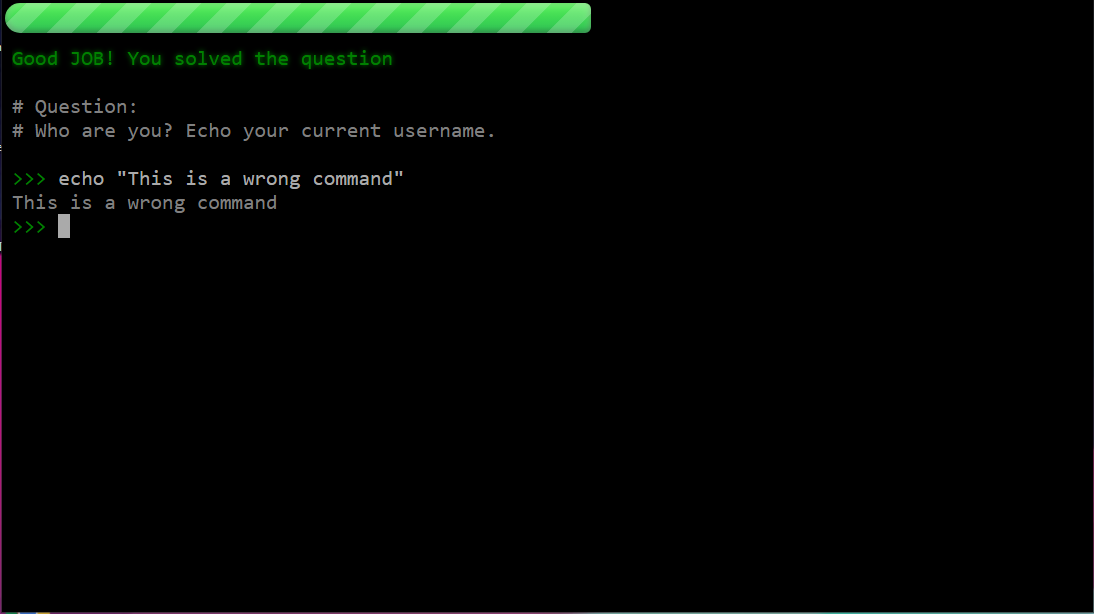
\includegraphics[width=\textwidth]{img/full_web.png}
    \caption{Beispielhafte Darstellung der Anwendung in der Fortschrittsanzeige-Bedingung (FA)}
\end{figure}

\subsubsection{Technische Implementation}
Bei der entwickelten Anwendung handelt es sich um eine interaktive Webanwendung, die sowohl auf Mobilgeräten als auch an einem klassischen Computer nutzbar ist. Die Anwendung besteht aus drei Komponenten:

\paragraph{Statische Webseite:}
Die Webseite basiert auf HTML, CSS und Javascript. Die graphische Darstellung einer Kommandozeile basiert auf dem jQuery Plugin \qq{jQuery Terminal Emulator}\footnote{https://terminal.jcubic.pl/}. Die Webseite kommuniziert Nutzerdaten und abgesetzte Befehle über eine REST-API mit dem Server. Die Webseite verfügt über keinerlei Anwendungslogik und stellt lediglich die empfangenen Daten des Servers dar. Für die gesamte Anwendung wurde ein dunkles Farbschema gewählt, das im Kern aus den Farben Grün und Schwarz besteht und einem Terminal ähnelt.

\paragraph{Server:}
Der Server ist in Python geschrieben und basiert auf dem Framework Flask\footnote{https://github.com/pallets/flask}. Der Server ist verantwortlich für die Nutzerverwaltung, die Nutzererkennung, das Ausführen und die anschließende Validierung abgesetzter Befehle sowie die Datenerfassung. Sämtliche Daten werden in einer MySQL-Datenbank gespeichert. Empfangene Befehle reicht der Server an den Executor weiter und nutzt dafür eine JSON-basierte REST-API. Der Server fungiert zusätzlich als Cache für bereits ausgeführte Befehle, damit jeder Befehl nur ein einziges Mal real ausgeführt werden muss.

\paragraph{Executor:}

  Da Konsolenbefehle kombinierbar sind, gibt es stets mehrere Antwortmöglichkeiten: Selbst einfache Fragen wie \textit{Geben Sie \say{Hello World} auf der Kommandozeile aus} haben diverse Lösungsmöglichkeiten, etwa:
  \begin{center}
      \verb|echo Hello World|
  \end{center}
  oder 
   \begin{center}
      \verb|echo hello world > t && cat t|.
  \end{center}
  Daher ist es nötig, die abgesendeten Befehle real auszuführen. Dazu wird jeder Befehl in einem eigenen Docker Container ausgeführt und die Ausgabe sowie mögliche Seiteneffekte mit der erwarteten Ausgabe abgeglichen. Diese Aufgabe übernimmt der Executor als separate Komponente. Dabei handelt es sich um eine simple Python API, die für das Starten, das Verwalten und das Löschen von Dockercontainern verantwortlich ist. Für jeden Befehl wird ein neuer Container gestartet und die Ausgabe des Befehls auf Korrektheit geprüft. Die Container basieren auf einem minimalen Python Image.


\subsubsection{Datenerfassung}
Während des Experiments werden unterschiedliche Daten erfasst, die sowohl der Auswertung des Experiments als auch dem Ausschluss von Mehrfachteilnahmen dienen:

\paragraph{Demographische Daten:}
Die in \ref{demography} dargestellten Fragen werden für jeden Nutzer in der Nutzertabelle gespeichert. Zusätzlich wird die jeweilige Experimentalbedingung in derselben Tabelle gespeichert.

\paragraph{Gerätespezifische Daten:}
Für jeden Nutzer wird die IP-Adresse sowie der User-Agent gespeichert, um Mehrfachteilnahmen zu identifizieren.

\paragraph{Nutzungsdaten:}
Während des Experiments werden unterschiedliche Daten erfasst, die der späteren Bewertung der Effektivität der einzelnen Maßnahmen dienen:

\begin{itemize}
	 \item abgesendete Befehle mit Zeitstempel
	 \item gelöste Aufgaben 
	 \item erreichte Abzeichen (nur für die Experimentalbedingung Abzeichen)
	 \item Feedback hinsichtlich der empfundenen Motivation (nur nach vollständiger Bearbeitung des Experiments)
\end{itemize}


\subsection{Pretest}\label{verlauf}
Vor der Veröffentlichung des Experiments wurde ein Pretest durchgeführt, der potentielle Fehler und Unklarheiten im Studiendesign aufzeigen sollte. Zusätzlich kann überprüft werden, ob die Studie grundlegend funktioniert. Im Rahmen des Tests wurden neben kleineren Fehlern wesentliche Probleme deutlich: Zum einen waren die Abzeichen deutlich zu unauffällig und wirkten laut Aussage der Teilnehmer wenig bis gar nicht motivierend. Aus diesem Grund wurden die Abzeichen größer und farbenfroher gestaltet. Zusätzlich wurde eine Animation abgespielt, sobald ein Abzeichen erreicht wurde. Außerdem gaben mehrere Teilnehmer an, dass die Fragen unverständlich und zu komplex seien. Dies hat dazu geführt, dass die Komplexität der Fragen reduziert wurde. Die so entstandenen Fragen lassen sich durch die Kombination von maximal zwei Befehlen lösen. Zusätzlich wurde eine Hilfsfunktion eingebaut, die durch den Befehl \textbf{help} aufrufbar ist. Außerdem wurde die Reaktionszeit der Anwendung, definiert als Zeitspanne zwischen dem Absetzen eines Befehls und der Anzeige des Ergebnisses, als sehr langsam empfunden. Daher wurde das Image des Containers verkleinert und auf die nötigsten Programme reduziert. Zusätzlich wurde ein Cache für bereits ausgeführte Befehle eingeführt. Die geschilderten Maßnahmen führen dazu, dass die Anwendung eine mittlere Reaktionszeit von 0.5 bis 2 Sekunden pro abgesetztem Befehl aufweist.


\subsection{Statistische Auswertung}
Die Gesamtspielzeit ergibt sich aus der Differenz des ersten und letzten abgeschickten Befehls. Zeitspannen von mehr als 30 Minuten ohne Nutzeraktivität - es wurde kein Befehl abgeschickt - werden als Inaktivität gewertet und von der Gesamtzeit abgezogen. Die aufgestellten Hypothesen werden mithilfe von t-Tests überprüft und die erforderlichen Voraussetzungen Normalverteilung und Harianzhomogenität werden separat geprüft. Die t-Tests werden durch eine einfaktorielle ANOVA Varianzanalyse erweitert, durch die sich die drei Versuchsgruppen miteinander vergleichen lassen.